\chapter{Contributions}\label{chap:con}


\section{Introduction}{\color{red} À discuter}

L'objectif de ce chapitre est de mener une étude sur les différentes structures de données nécessaires aux futurs algorithmes de visualisation. Dans une première partie, nous nous intéresserons à l'opération d'accès à une caractéristique ou d'une donnée d'une boîte ainsi qu'à l'occupation mémoire de cette dernière. Il s'appuie sur le document de spécification (cf. \ref{sec:spe}). Ce document sur les calculs de complexité seront réalisés selon le paramètre $n$  représentant le nombre de boîtes, et $d$ est le nombre de dimensions du problème. Le nombre de boîtes réellement utilisées dans le pavage est représenté par $N$. 


La seconde partie est consacrée à la la réalisation du logiciel de visualisation. Trois difficultés majeures apparaissent. La première est bien entendu la gestion d'une très grande quantité de boîtes lors de l'affichage. Il est en effet nécessaire d'offrir un accès rapide aux informations des boîtes dans la fenêtre. La seconde est la gestion des filtres sur ces mêmes boîtes. Et le troisième apparait lors du changement des variables étudiées (changement des dimensions visualisées). Dans cette section, nous chercherons d'avantage à apporter une solution pour les problèmes de temps d'accès et de changement de variables. Il est en effet probable que la gestion des filtres soit effectuée par une structure différente.





\section{Définition de la boîte}
C'est l'entité atomique du pavage. Les accès à ses attributs sont donc cruciaux. On rappelle qu'une boîte est définie de la manière suivante : 
\begin{itemize}
\item 
  Un identifiant : soit des chaînes de caractères (IDStr) respectant un format précis (cf. 1.1 du document de spécifications), soit des entiers positifs (IDInt).
\item
  Une liste de coordonnées dans l'ordre des variables définies en entête. Une liste de type \verb+Interval+.
\item
  Une liste des caractéristiques, dans l'ordre et selon les types définis en entête.
\end{itemize}
Ces données seront régulièrement requises lors de la mise en œuvre des algorithmes nécessaires à la visualisation. Il est donc important que leurs accès soient rapides, voire directs. Pour le cas de l'identifiant, s'agissant d'une simple \verb+String+ le problème de la structure à utiliser ne se pose pas. Pour la liste des coordonnées en revanche, il s'agit d'une séquence finie de données. Plusieurs possibilités sont alors envisageables : 

\begin{itemize}
\item
  Un tableau : L'accès à une coordonnée est direct. Les opérations d'ajout et de suppression sont en revanches coûteuses pour les tableaux dynamiques ($O(n)$).
\item
  Une liste : Si l'accès à une coordonnée n'est pas direct ($O(n)$), les opérations d'ajout et de suppression sont en temps constant.
\item
  Une table de hachage : Coûteuse si la fonction de hachage n'est pas appropriée, une table de hachage propose cependant un accès en $O(1)$.  Cependant le phénomène de collisions (mauvaise répartition des clefs entrainant un conflit entre deux valeurs) est à prendre en considération :

\begin{description}
\item[Implémentation avec un tableau dynamique] Une telle structure permet de garantir un accès en temps constant. Cependant chaque collision va doubler l'occupation mémoire du tableau. Or même si la fonction de hachage est bonne, il est possible d'avoir au moins une collision, ce qui aurait pour conséquence une perte de l'espace mémoire qui se répercuterait sur chaque boîte.
\item[Gestion des collisions avec chaînage] Contrairement à la structure précédente, cette méthode permet de ne pas occuper trop d'espace en chainant les éléments entrants en collision. Malheureusement la complexité en pire cas des opérations d'accès passe en $O(n)$. En revanche, grâce à une bonne fonction de hachage, on accèdera généralement en temps constant sans contre coût mémoire. 
\end{description}

Le passage en revue de ces différentes structures écarte la liste et la table de hachage implémentée par un tableau dynamique. En effet les performances des opérations d'accès de la liste ne sont pas raisonnables. De même l'implémentation d'une table de hachage par un tableau dynamique risque d'entrainer une perte de mémoire trop importante.
%\item
 % Une TreeMap \cite{TreeMap}. Implémentation de base des arbres rouges noirs, cette map a la particularité de posséder des clefs triées. Ainsi les complexités de plusieurs opérations telle que l'accès en $O(\log{n})$. Dans le cas d'un grand nombre de valeurs à stocker, il est plus performant de construire la TreeMap à partir d'une HashMap.

\end{itemize}

%La création d'une boîte a alors une complexité en $O(d)$. De plus l'accès aux différents attributs de la boîte (identifiant, liste des coordonnées) sera en $O(1)$.

\subsection{Généricité des caractéristiques}
Un problème majeur apparaît pour l'instanciation des boîtes. On rappelle qu'une caractéristique à plusieurs types (\verb+String+, \verb+Number+ ou \verb+Interval+). Plusieurs solutions sont envisageables : 
\begin{itemize}
\item
  Une Map unique contenant des \verb+String+ stocke les différentes caractéristiques de la boîte. On aura casté les attributs \verb+Number+ ou \verb+Interval+ en \verb+String+. Il sera alors nécessaire, pour chaque futurs accès, d'effectuer un cast dynamique. On rajoute alors une constante supplémentaire à la complexité de cette opération. 
\item 
Trois tableaux (un pour chaque type) au sein d'une boîte. Trois Maps (une pour chaque type) «générales» au niveau du pavage. La clef d'une map est l'id de la caractéristique et la valeur de la map son indice dans le tableau concret. La boîte peut alors retrouver la valeur de la caractéristique au sein de son tableau.
\item 
  Chaque boîte possède trois Maps pour ces trois types de caractéristiques. 
\end{itemize}


\section{Pavage}
\subsection{Problématique}
%L'outil de visualisation peut charger un fichier entrée de manière dynamique ou non. Nous nous plaçons ici dans le cadre où cette option de chargement dynamique n'est pas activée. \\ 
%L'outil va lire séquentiellement chaque ligne du fichier d'entrée.
Le cahier de spécification exige de l'outil la capacité à charger un pavage de taille non déterminée. Si le nombre de boîtes sera en pratique nécessairement borné (limite mémoire de la machine), il faut cependant répondre à cette attente en proposant une structure de stockage capable de supporter un très grand nombre de boîtes. De plus l'outil doit être en mesure de fournir régulièrement des listing spécifiques de boîtes. Par exemple pour afficher la liste de celles concernées par un \emph{filtre} (cf. \ref{sec:spe} section 1.2, 5\up{ème} point). La structure du pavage doit être en mesure de répondre de manière efficace à des requêtes de séquences de boîtes selon un ordre particulier. La structure du pavage doit être aussi en mesure de répondre efficacement à la structure  de visualisation graphique (fournir rapidement les nouvelles boîtes dans le champs de visualisation, lors d'une rotation de caméra par exemple). Quelles structures de données et quelles stratégies choisir face à de telles exigences ?  %Ce chapitre débute par de le passage en revue de différentes structures de données potentielles. % La création de la structure de stockage débute par la lecture séquentielle du fichier d'entrée (cf section 1  du document de spécification). Plusieurs options apparaissent à cette étape, faut-il par exemple :



\subsection{\'Etude de structures}

\paragraph{Vector :} Collection de données à accès direct par indice. Le nombre de boîte étant donné dans l'entête du fichier d'entrée, une implémentation par un tableau statique proposerait une complexité en temps égale à $O(n)$ pour l'opération de stockage du pavage. Si l'accès à une boîte à partir de son indice serait direct, l'opération de recherche en revanche aurait une complexité en temps égale à $O(n)$. 

\paragraph{Dictionnaire :} Collection de données à accès direct par clef. Dans l'hypothèse de posséder une fonction de hachage ne provoquant pas de collisions, une implémentation par une fonction de hachage propose une complexité en temps égale à $O(n)$ (à nouveau grâce à la connaissance du nombre de boîtes dans l'entête du fichier d'entrée).


%Le nombre potentiellement très grand de boîtes élimine d'emblée la possibilité de choisir une HashMap. En effet même si la fonction de hashage est judicieusement choisie, l'occupation mémoire requise serait bien trop importante. Les listes ne sont pas  appropriées ici. Une complexité en $O(n²)$ pour un accès à une boîte n'est pas raisonnable.
\clearpage
\paragraph{Arbre binaire}
L'utilisation d'un arbre binaire de recherche pour la création de $n$ boîtes aurait une complexité en temps égale à $O(n²)$ en pire cas. En effet il s'agit du cas où les boîtes arriveraient triées selon l'ordre inverse de celui que l'on souhaite. Ce critère d'ordonnancement des boîtes peut varier (Id, caractéristique «temps de calcul», borne inférieur d'une variable, \dots{}). Il faudrait alors effectuer $(p-1)$ comparaisons, pour chaque boîte :  $\sum_{p=2}^{n}(p-1)$  Soit une compléxité en temps égale à $O(n)=\frac{1}{2}n²-\frac{1}{2}n$. Cependant dans le meilleur des cas, cette opération a une complexité en temps égale à $O(n\log{n})$. La création d'un pavage composé de $n$ boîtes à $d$ dimensions aurait alors une complexité en temps égale à: $O(d \times n\log(n))$.

\begin{figure}[htbp]
  \centering
  \includegraphics[scale=0.60]{img/binTree}
  \caption{arbre binaire}
  \label{fig:abtree}
\end{figure}
L'arbre binaire était équilibré par définition, la complexité en temps de son opération de recherche est en $O(\log_2{n})$ (hauteur de l'arbre).
   


%http://www.enseignement.polytechnique.fr/profs/informatique/Luc.Maranget/421/poly/arbre-bin.html
%\clearpage
\paragraph{Arbres a-b}
Il s'agit d'un arbre de recherche avec les propriétés suivantes :
\begin{itemize}
\item
  $a\leq2$ et $b\leq 2a−1$ deux entiers.
\item
  La racine a au moins 2 fils (sauf si l'arbre ne possède qu'un nœud) et au plus b fils.
  Les feuilles sont de même profondeur.
\item
  Les autres nœuds internes ont au moins a et au plus b fils.
\end{itemize}

\begin{figure}[h!tbp]
  \centering
  \includegraphics[scale=0.40]{img/abtree}
  \caption{a-b arbre}
  \label{fig:abtree}
\end{figure}

L'avantage des arbres a-b est que leurs hauteurs  sont comprises entres les valeurs suivantes : $ \dfrac{\log{n}}{\log{b}}   \leq h  < 1 + \dfrac{\log{n/2}}{\log{a}}$. Ainsi les opérations d'insertion ne seraient plus en $O(n\log{n})$ mais en $O(\log{n})$. La création d'un pavage composé de $n$ boîtes à $d$ dimensions aurait alors une complexité temporelle en $O((n\times d)\log(n))$. La recherche d'un boîte quant à elle aurait une complexité en $O(\log{n})$.

\paragraph{}
Ce passage en revue de ces différentes possibilités permet, pour certaines d'entre elles, de sugérer un usage dans certaines conditions.  En effet les structures telles que les \emph{dictionnaires} ou les \emph{vectors} ne sont pas recommandables pour le stockages du pavage. On peut notamment leurs reprocher le coût trop élevé de l'opération de recherche de la structure \emph{vector}. Quant aux \emph{dictionnaires}, ses performances sont restrictives à l'existence d'une fonction de hachage ne provoquant pas de collisions. 

Les structures arborescences ont l'atout de pouvoir stocker et manipuler un grand nombre d'entités par des opérations ayant, la plupart du temps, des complexités en temps d'ordre logarithmique. On peut cependant envisager une utlilsation de structures à accès direct (\emph{vectors}, \emph{dictionnaires}) en parallèle de structures arborescences dans le cadre de certaines opérations (recherche d'une liste de boîtes pour l'application d'un \emph{filtre}, d'une vue, \dots{}). En revanche, le maintien de la cohérence entre une structure contenant le pavage et ces structures \og secondaires \fg{} introduit une redondance et donc un coût en mémoire.

\section{Stockage des boîtes et visualisation}

\subsection{\'Etude d'une solution possible : le QuadTree}
\paragraph{}Une des solutions qui pourrait permettre une visualisation fluide du pavage tout en répondant au document de spécifications serait de représenter le pavages sous une forme de QuadTree pour deux dimensions ou OcTree pour trois dimensions.
\begin{figure}[htbp]
\centering
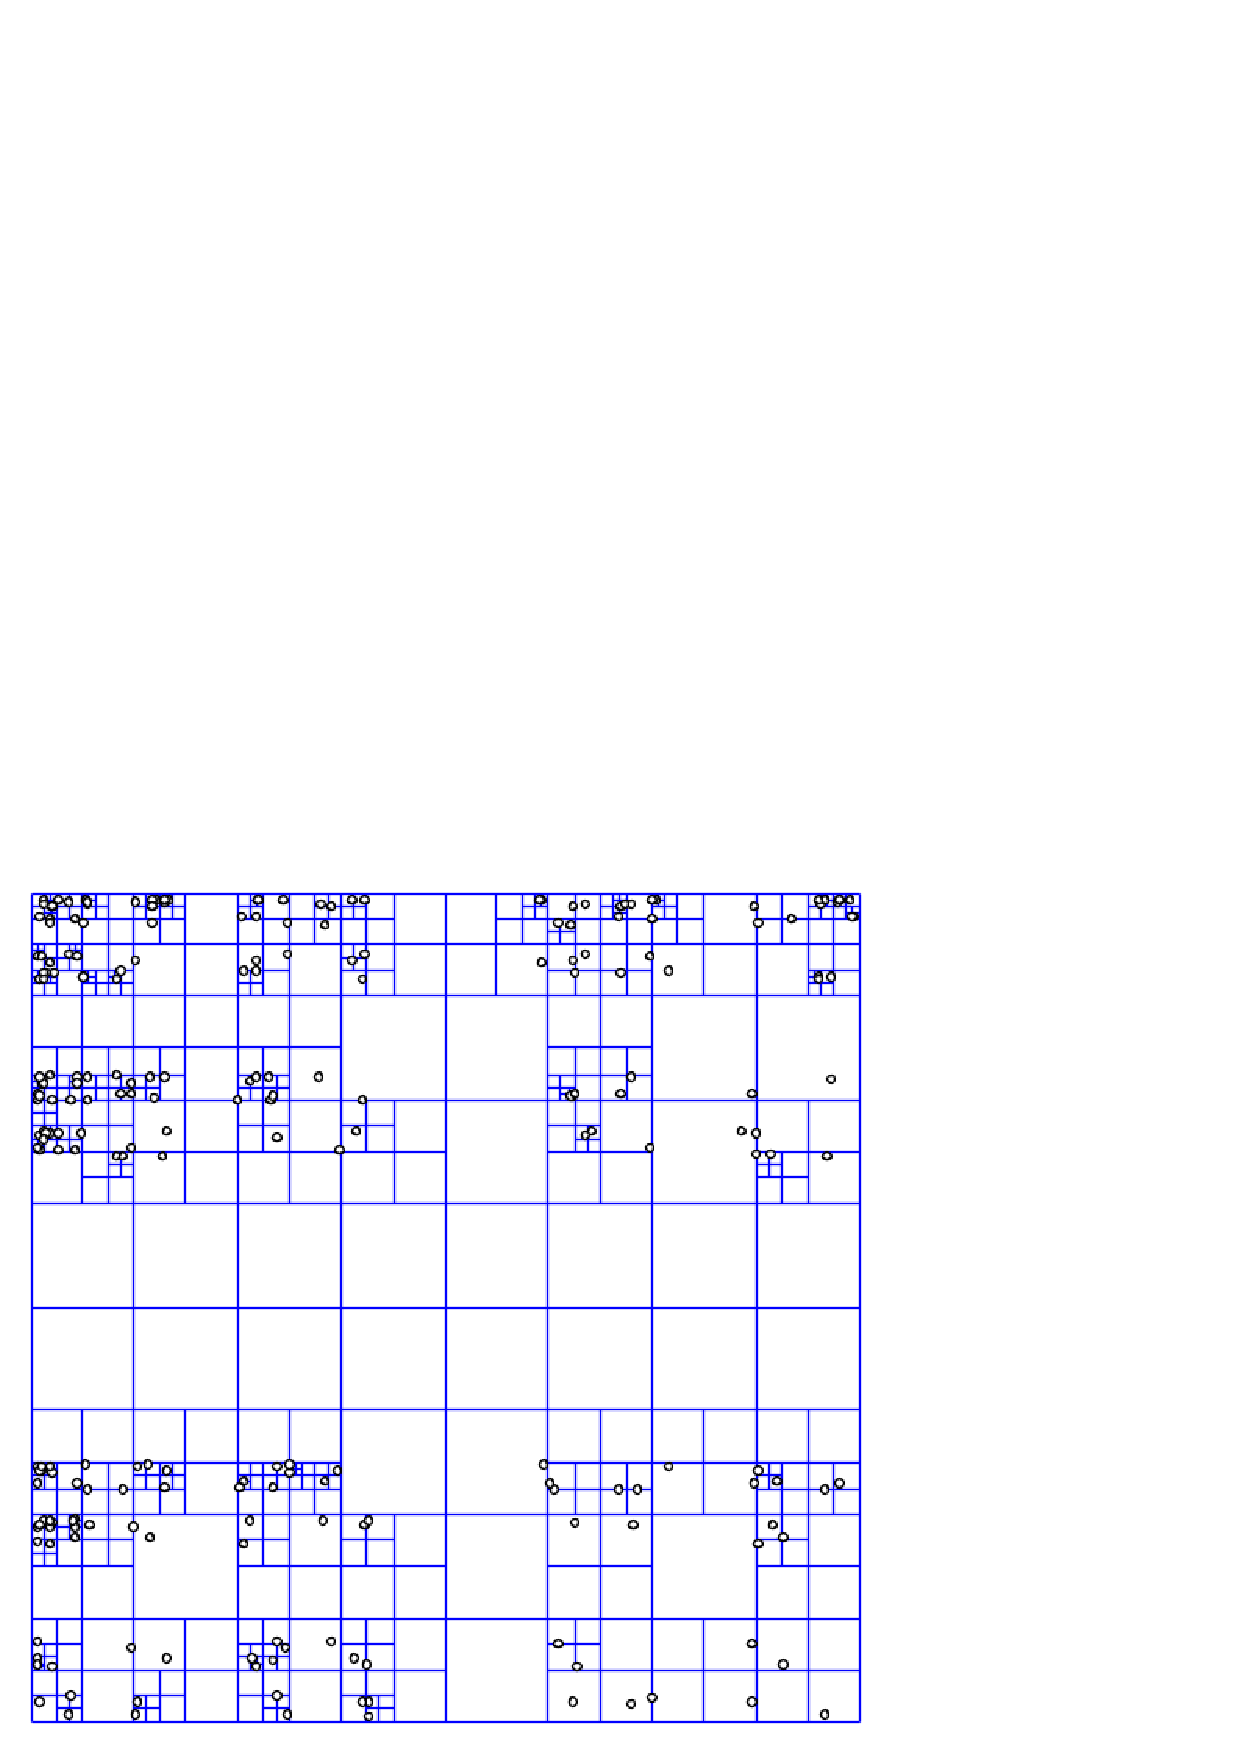
\includegraphics[scale=0.50]{img/quadtree}
\caption{Représentation d'un QuadTree où les données sont des points}

\end{figure}

Le QuadTree consiste à découper récursivement un espace fini en deux dimensions en quatre parties égales. Chacune de ces parties sont stockées dans une cellule. On itère ce mécanisme sur chacune de ces cellules jusqu'à isoler spatialement les éléments recherchés.

Cette structure pourrait être utilisée pour déterminer la position des boîtes dans l'espace.

\paragraph{}L'algorithme permettant de partitionner est récursif. Dans le cas récursif, l'algorithme divise une cellule en quatre et itère sur chacune des sous cellules. Dans le cas d'arrêt on ne subdivise plus. Nous décrivons par la suite l'ensemble des cas de récursions et d'arrêts pour la division d'une cellule donnée. Les images jointes au texte sont des représentations des différents cas dans lesquels les cadres rouges sont des boîtes solutions et les cadres noirs une cellule du QuadTree. Vous trouverez une classification visuelle dans la table \ref{tab:algo}.
\begin{enumerate}
\item Cas d'arrêts : 
\begin{enumerate}
\item La cellule fournie est entièrement inclus dans une boîte.
\label{enu:quad1}
\item La cellule fournie contient entièrement une seule boîte.
\label{enu:quad2}
\item La cellule fournie contient en partie une seule boîte.
\label{enu:quad3}
\item La cellule fournie n'intersecte aucune boîte.
\label{enu:quad4}
\item La cellule fournie ne peux plus être subdivisé car on a fourni une taille minimale pour les espaces.
\end{enumerate}
\item cas de récursions :
\begin{enumerate}
\item La cellule fournie intersecte plusieurs boîtes.
\label{enu:quad5}
\end{enumerate}
\end{enumerate}

\begin{table}[htbp]
\centering
 \begin{tabular}{|c|cccc|}
  \hline
  Cas de récursion &  \ref{enu:quad5}.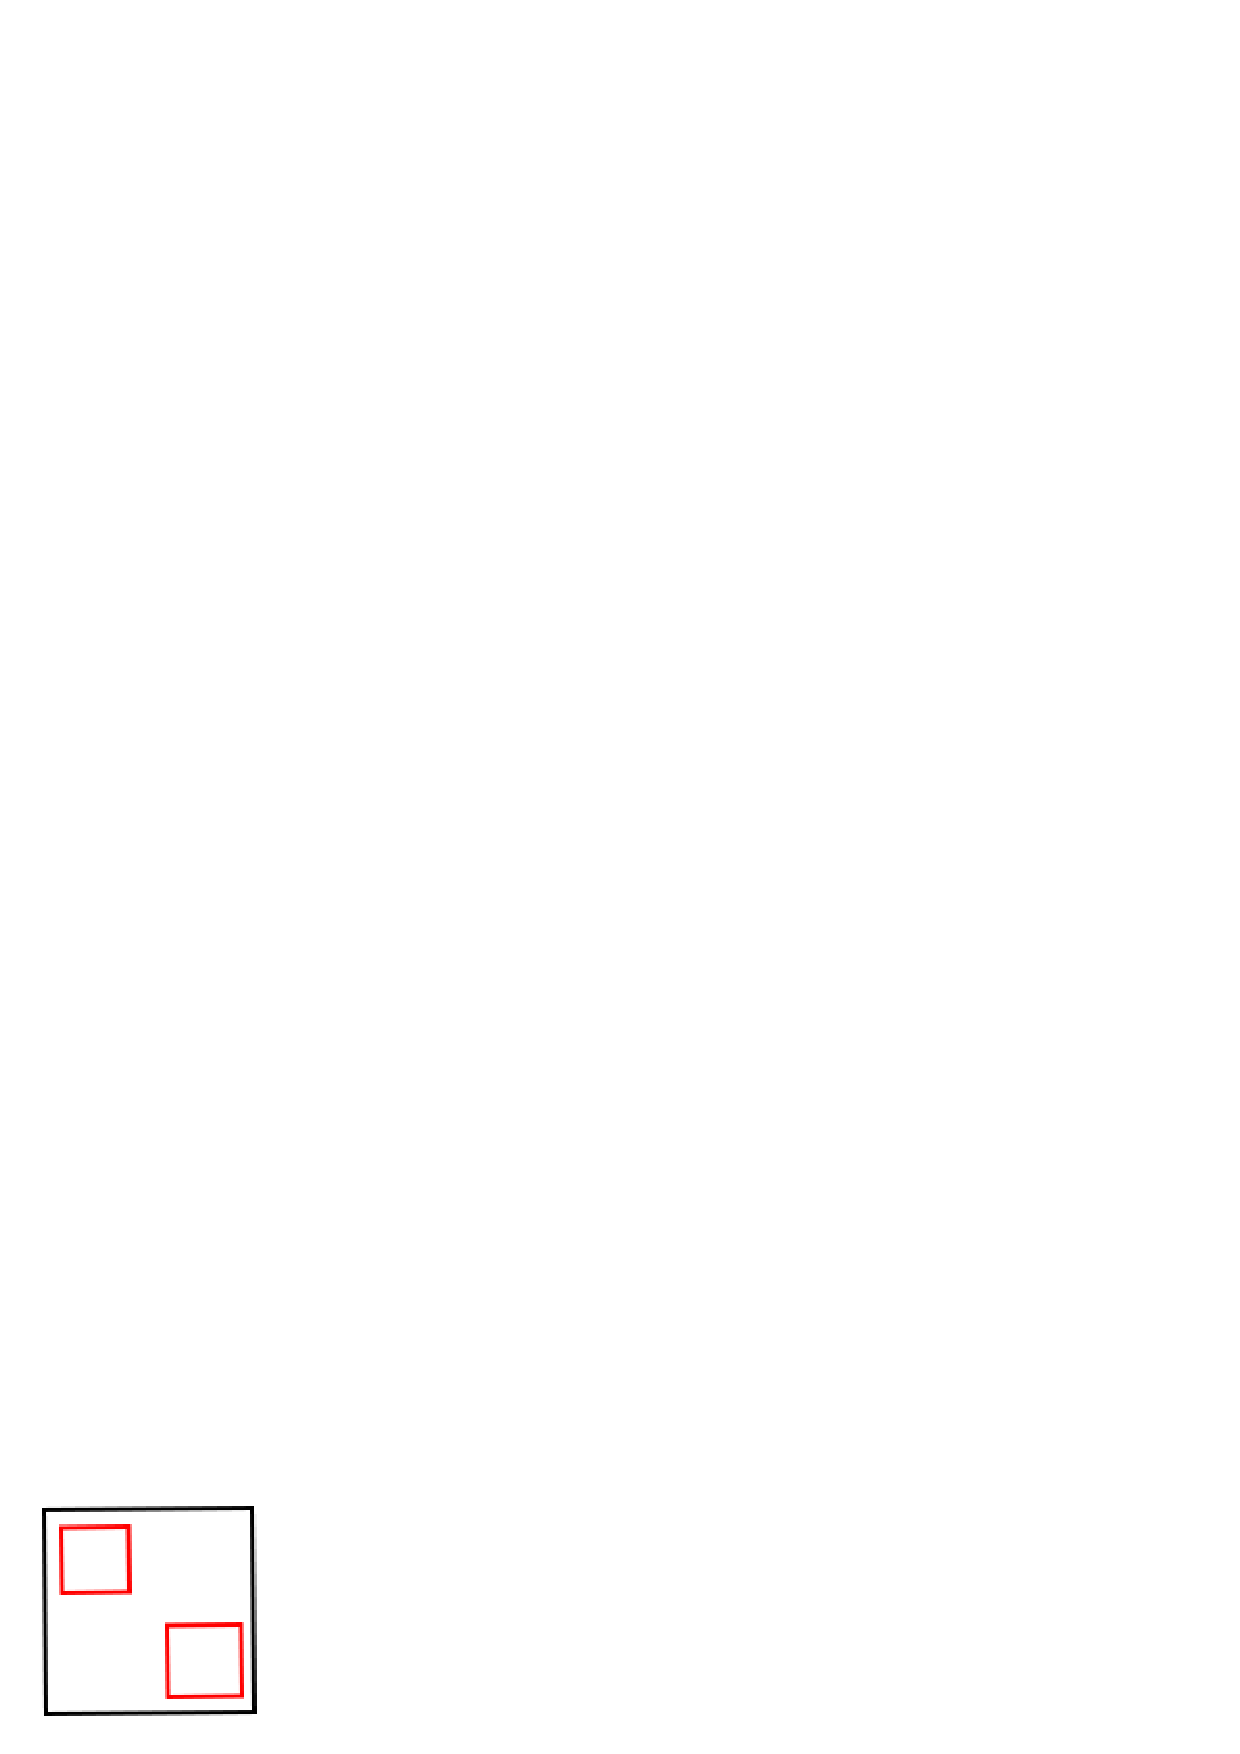
\includegraphics[scale=0.20]{img/QT4}&  \ref{enu:quad5}.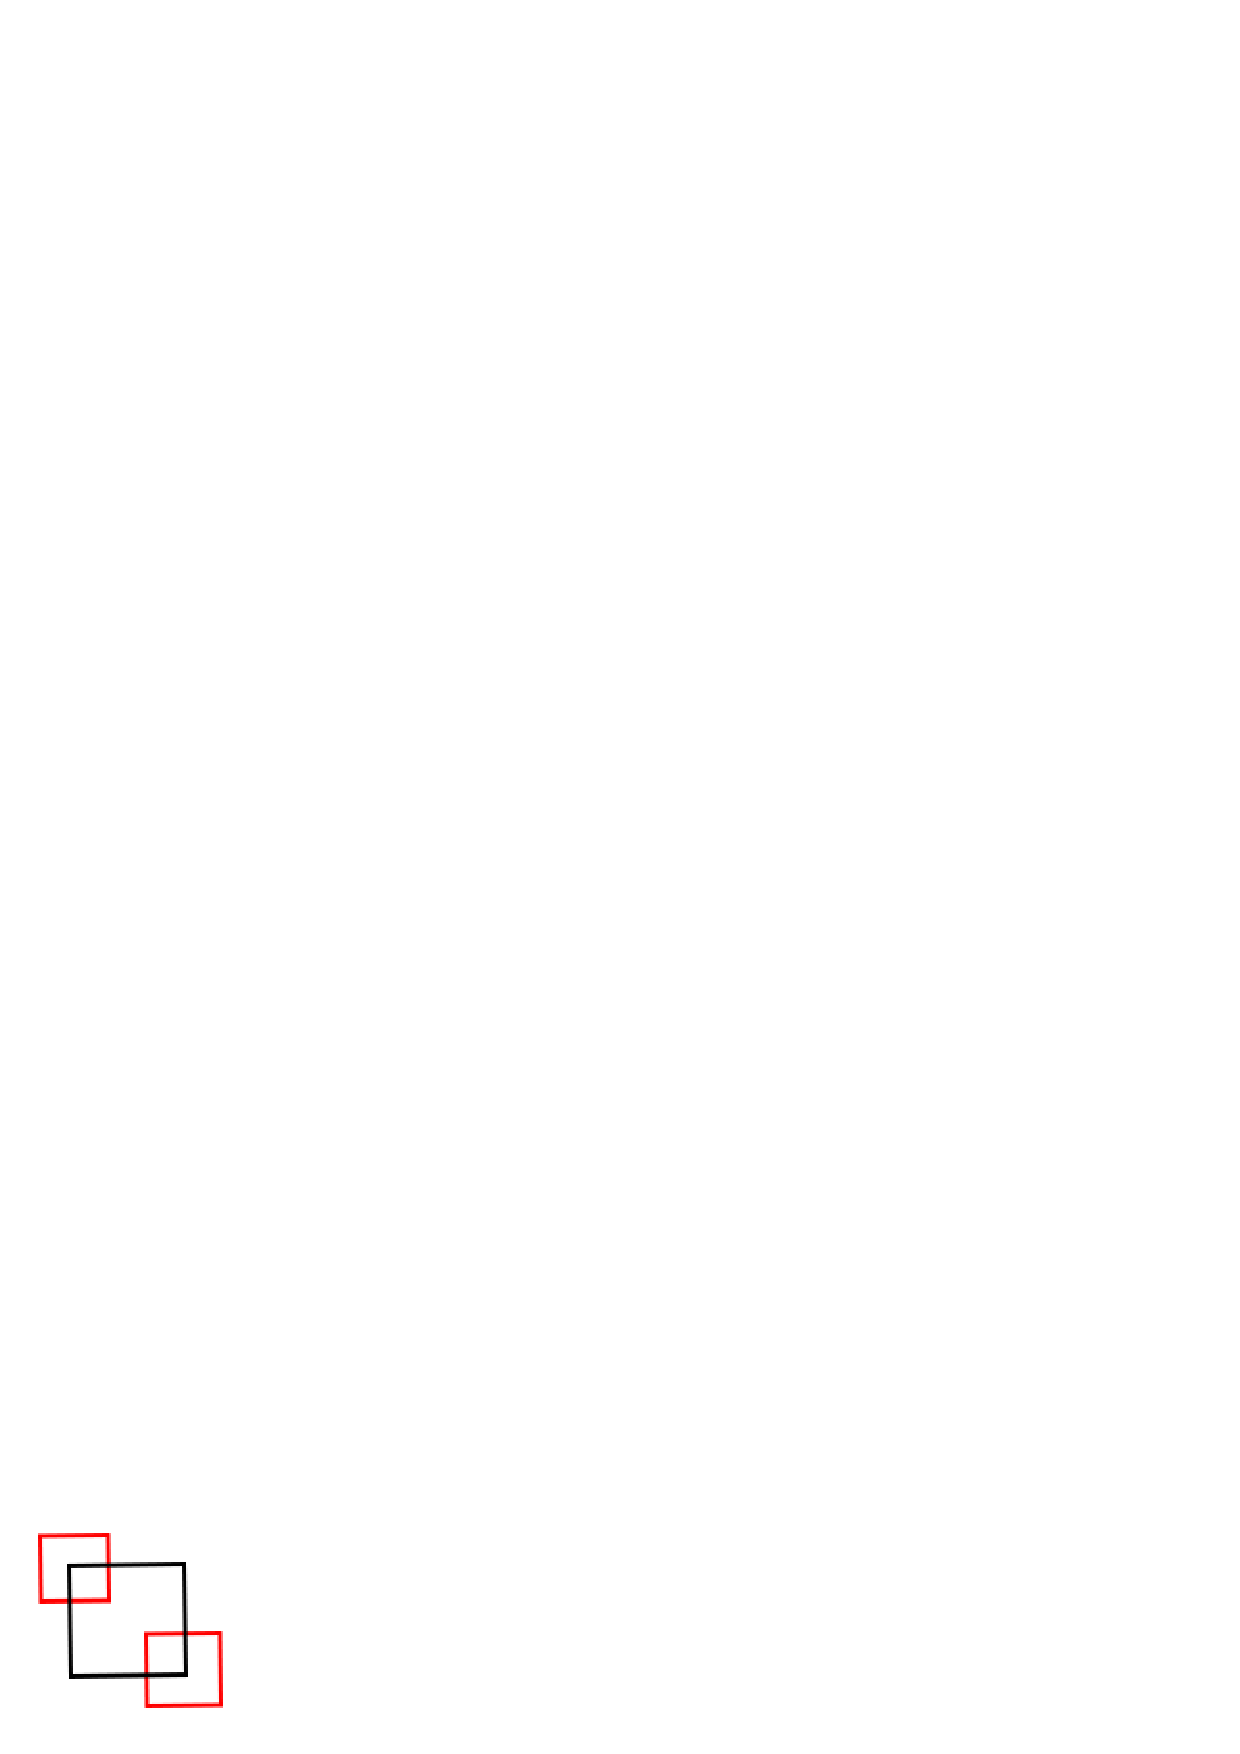
\includegraphics[scale=0.20]{img/QT5}& &\\
  \hline
  Cas d'arrêt&  \ref{enu:quad1}.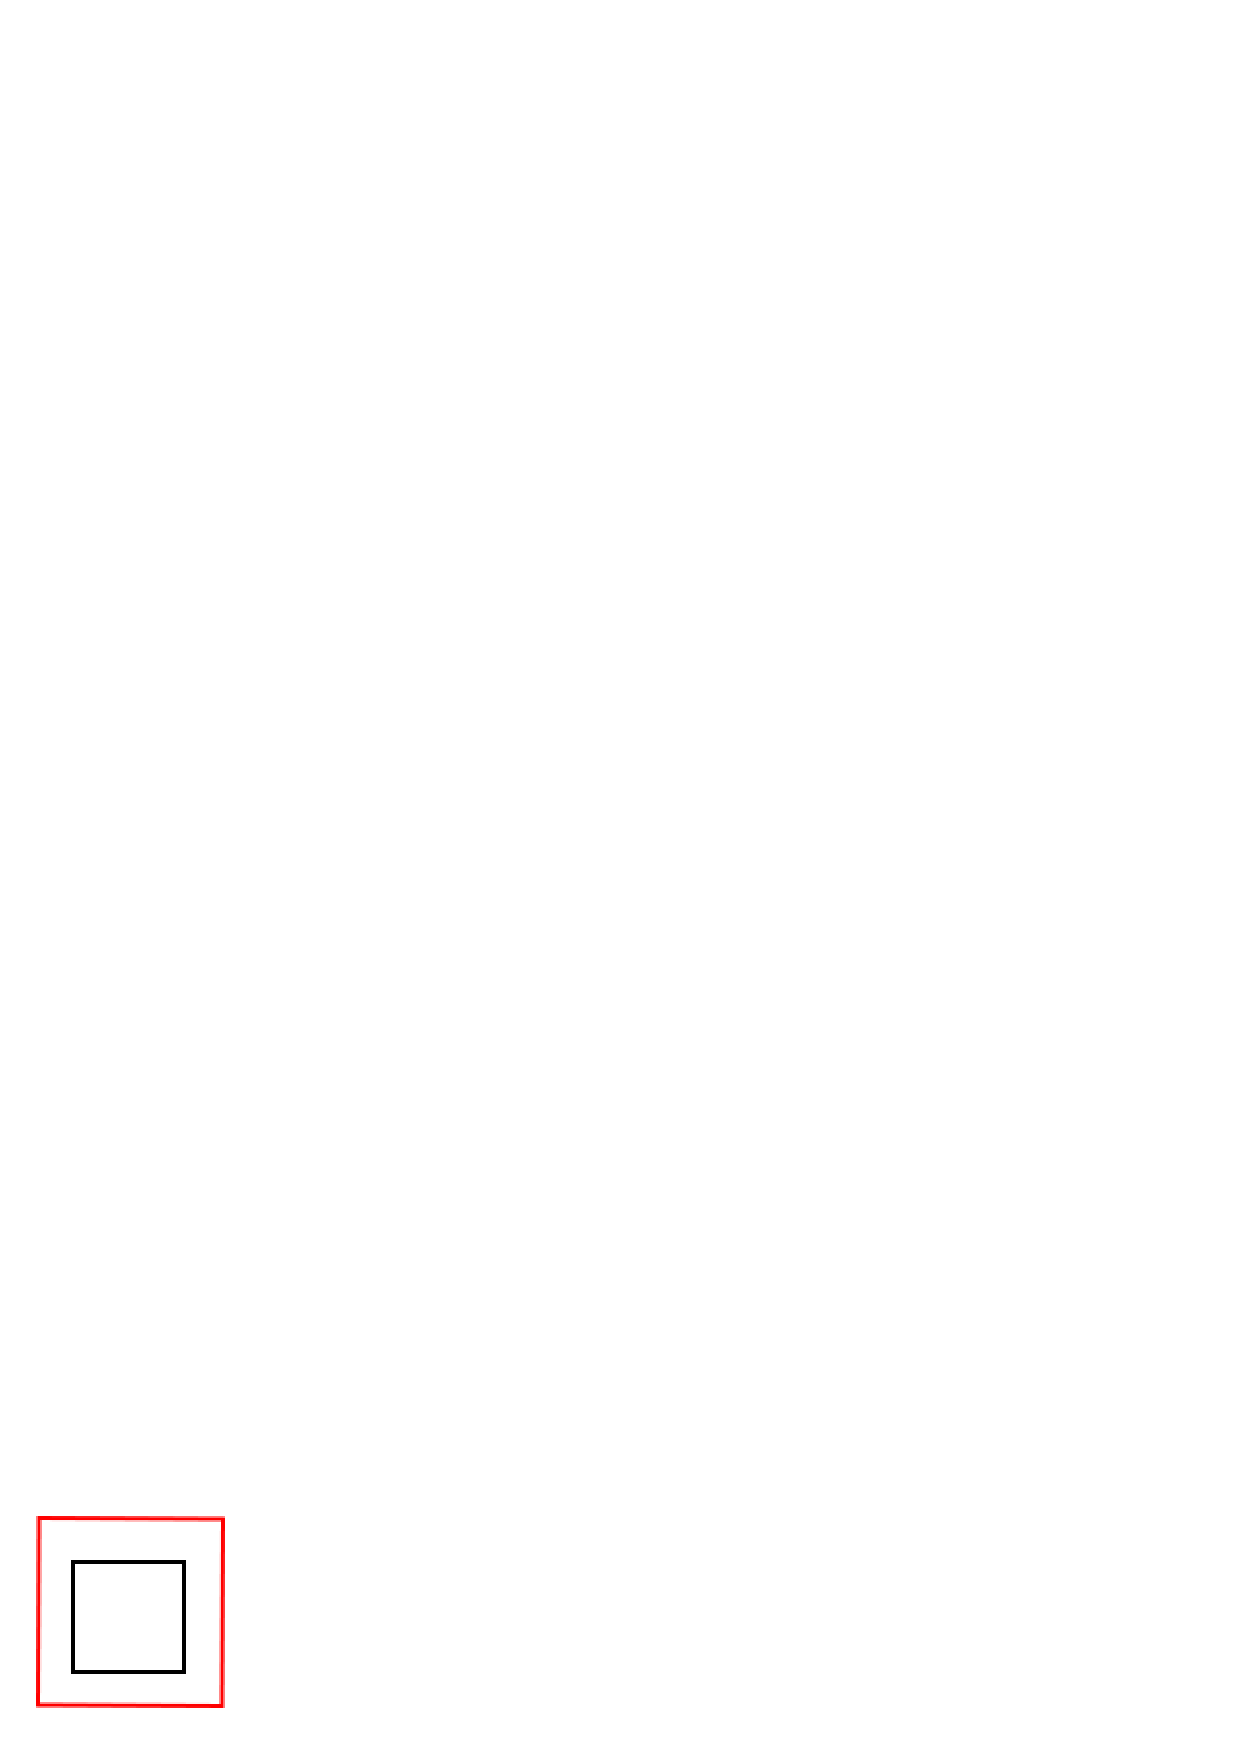
\includegraphics[scale=0.20]{img/QT1}&  \ref{enu:quad2}.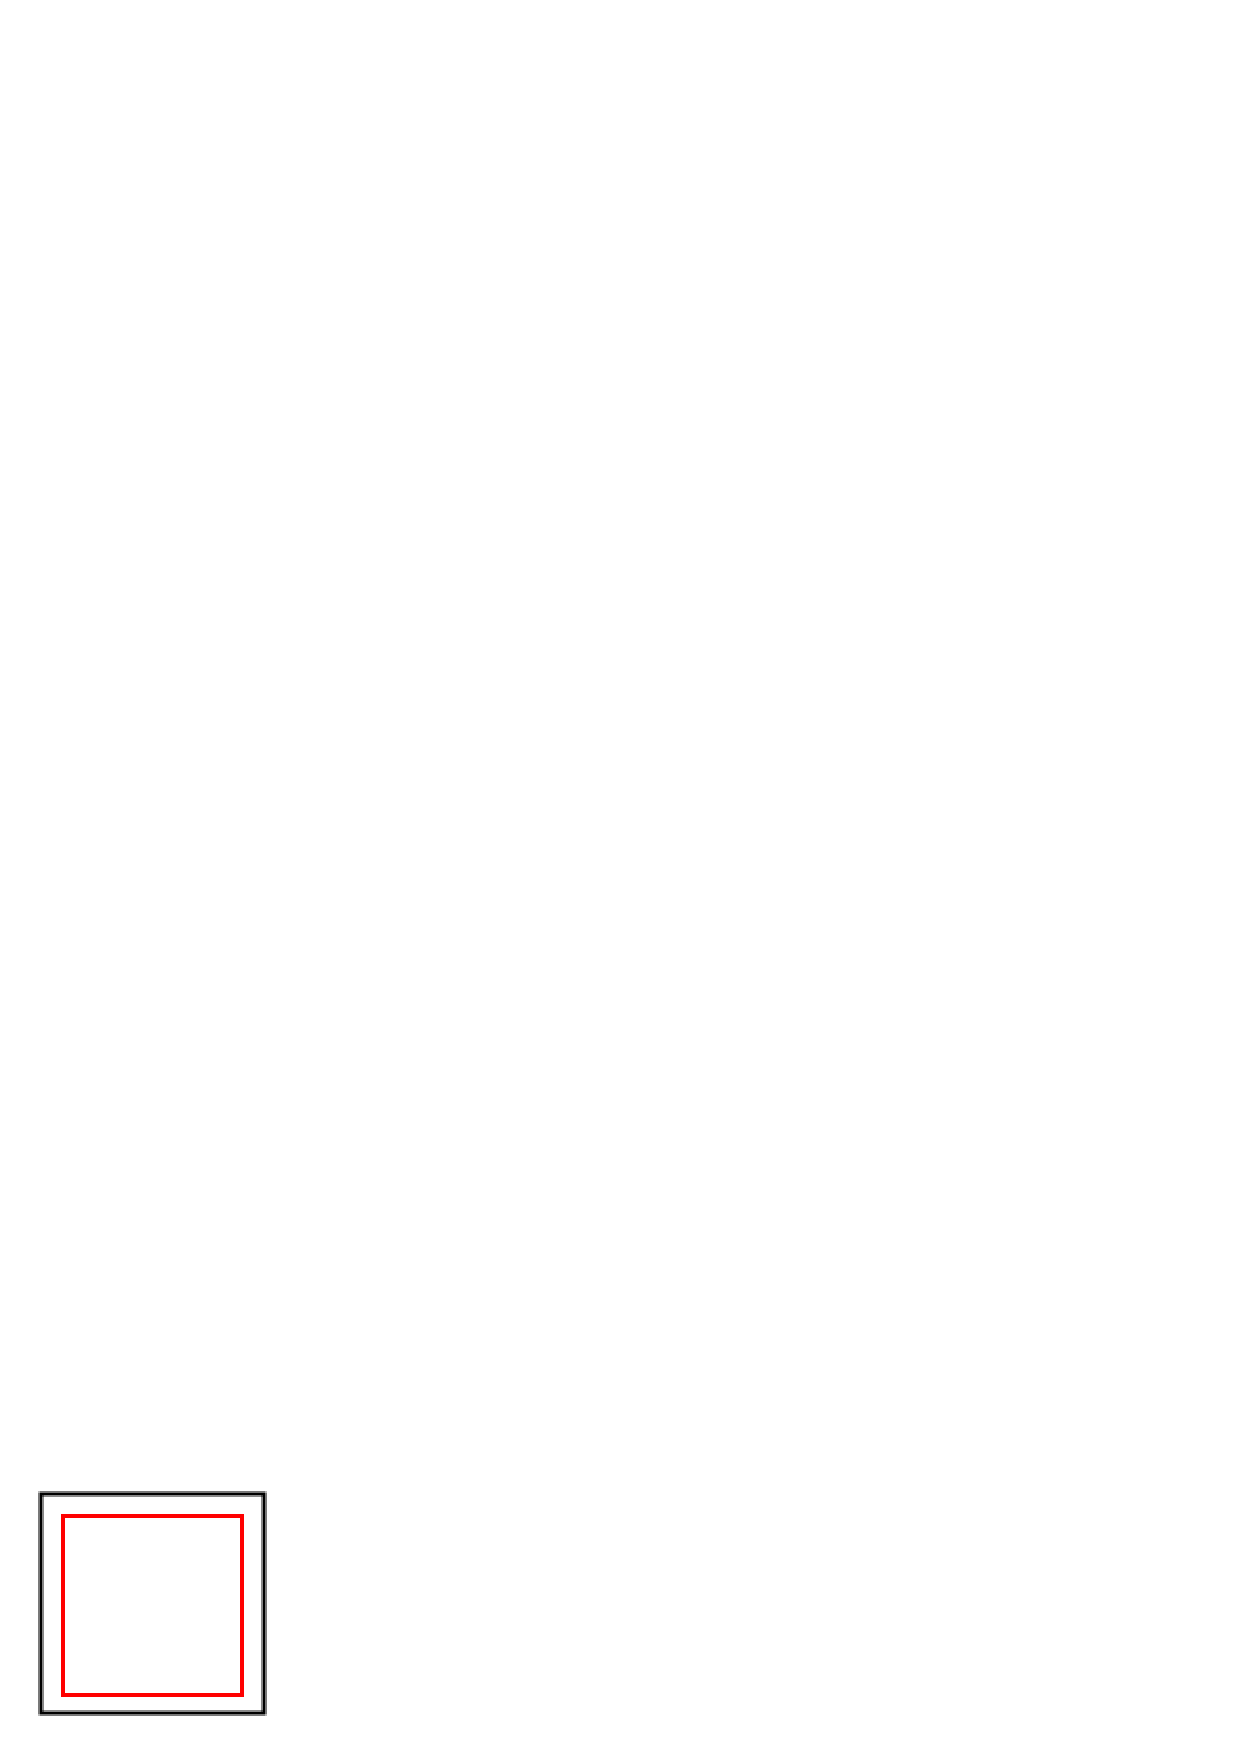
\includegraphics[scale=0.20]{img/QT2}&  \ref{enu:quad3}.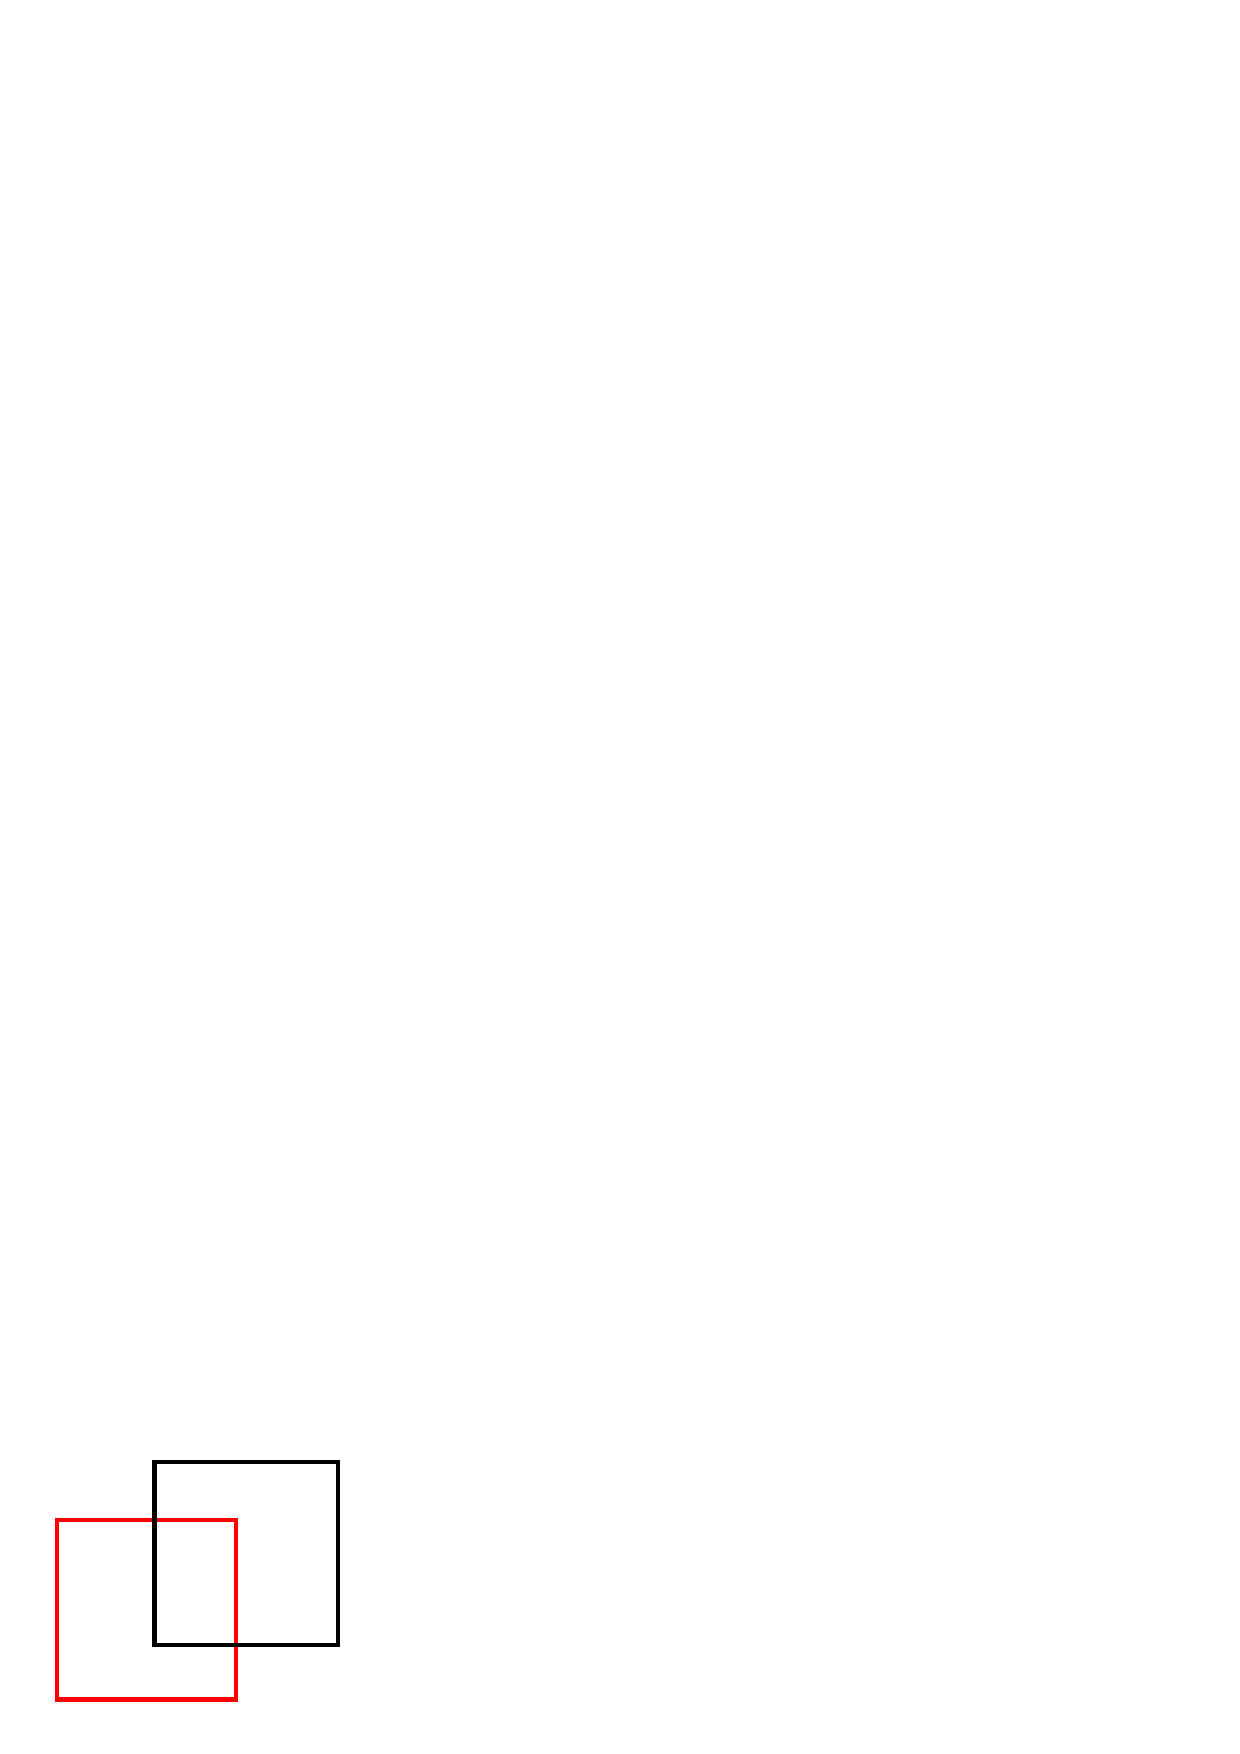
\includegraphics[scale=0.20]{img/QT3}&  \ref{enu:quad4}.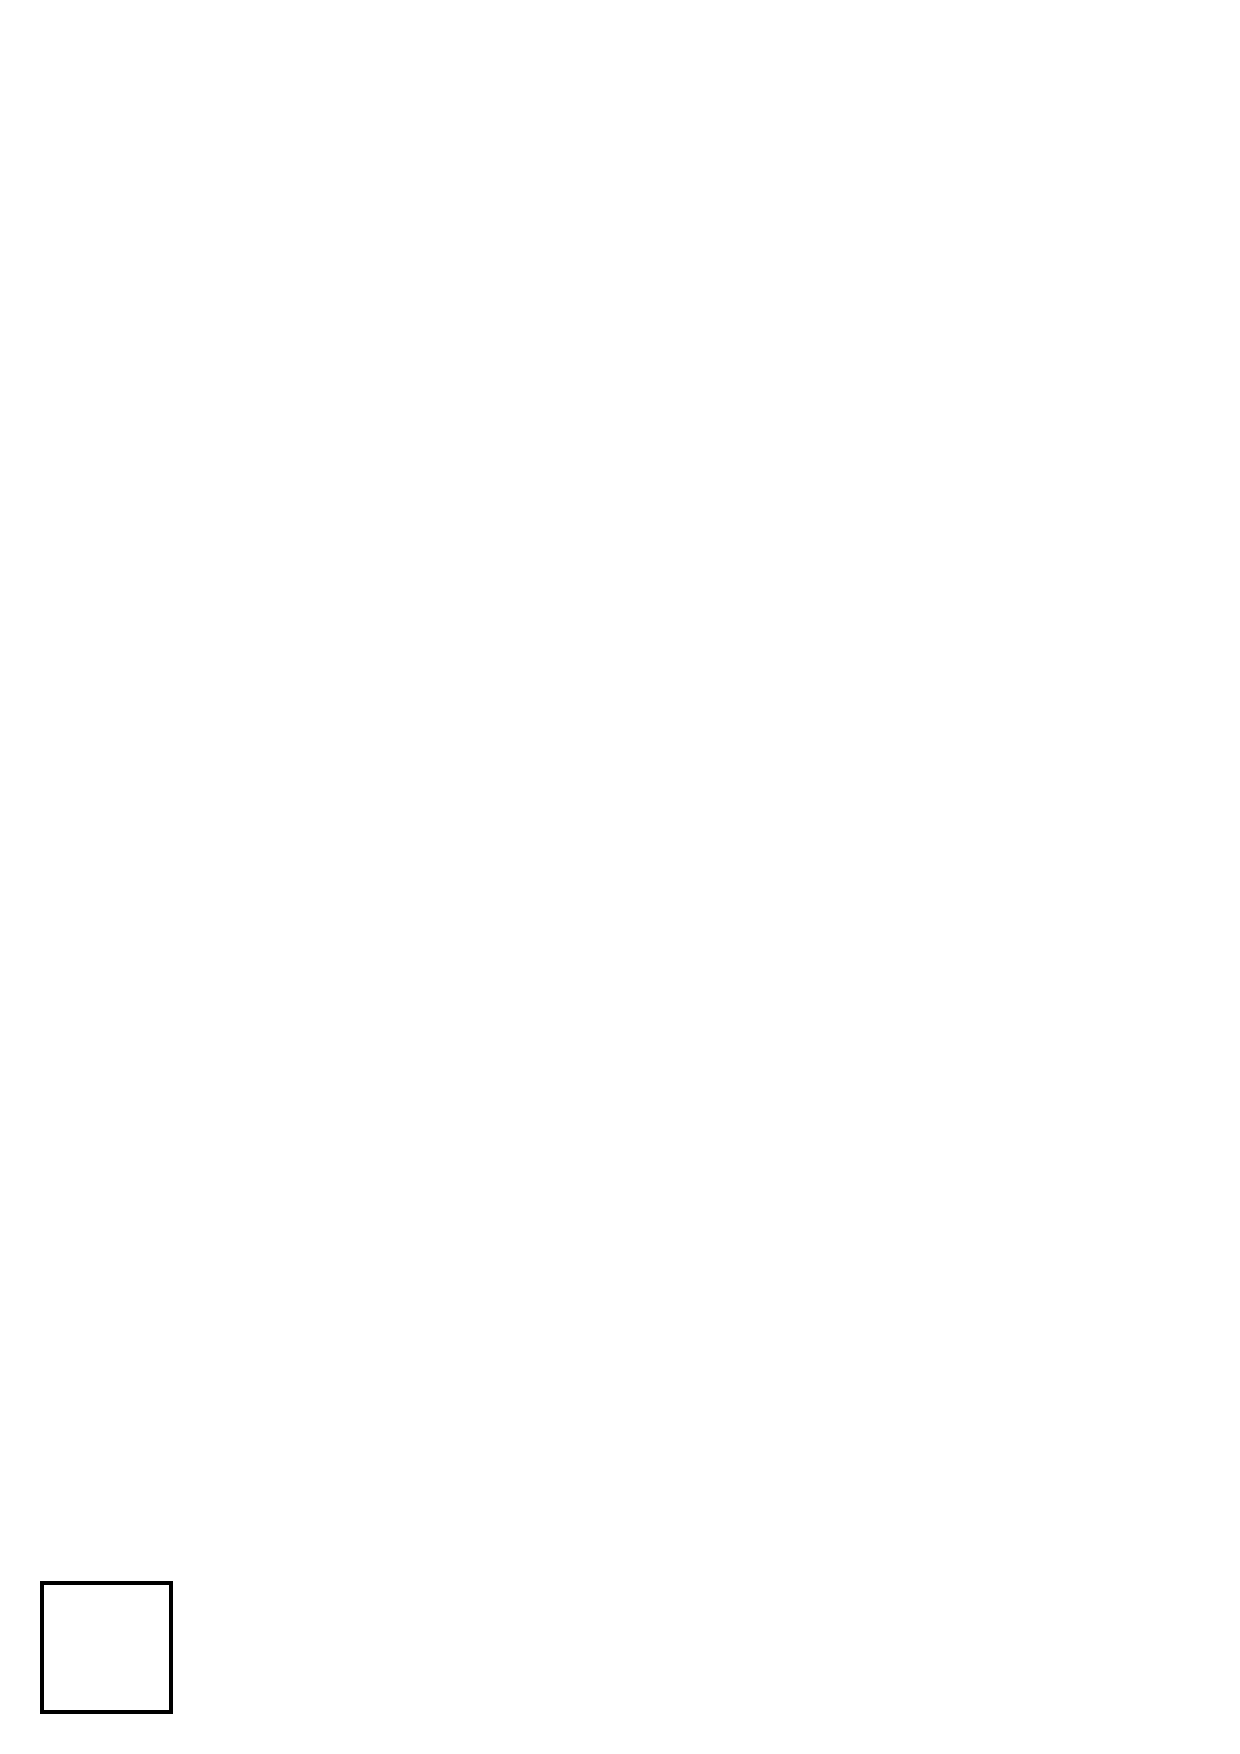
\includegraphics[scale=0.30]{img/QT6}\\
  \hline
 \end{tabular}
 \caption{Classification visuelle des cas d'arrêts et de récursions}
\label{tab:algo}
\end{table}


L'OcTree repose sur le même principe mais étendu à trois dimensions. Une cellule est donc découpée en huit parties à chaque fois.

\paragraph{Avantage de cette méthode}Cette structure est particulièrement intéressante pour la visualisation du pavage. En effet pour une fenêtre de visualisation donnée, il est très simple et rapide d'extraire la sous-arborescence correspondante à la fenêtre visualisée et permet aussi de ne pas afficher les objets trop petits. 

De plus il serait possible de créer une structure reposant sur le même principe que le QuadTree mais étant $k$-dimensionnelle\footnote{$k$ étant la dimension du problème fourni à RealPaver.}. Chaque espace peut alors être potentiellement subdivisé en $2^k$ sous-espaces. Cette structure permettrait d'éviter de recalculer l'arbre à chaque changement de variables de visualisation. On évite par ailleurs le cas de superposition de boîtes pour lequel l'algorithme n'est plus efficace (cf : figure \ref{fig:superpos}).
\begin{figure}[htbp]
\centering
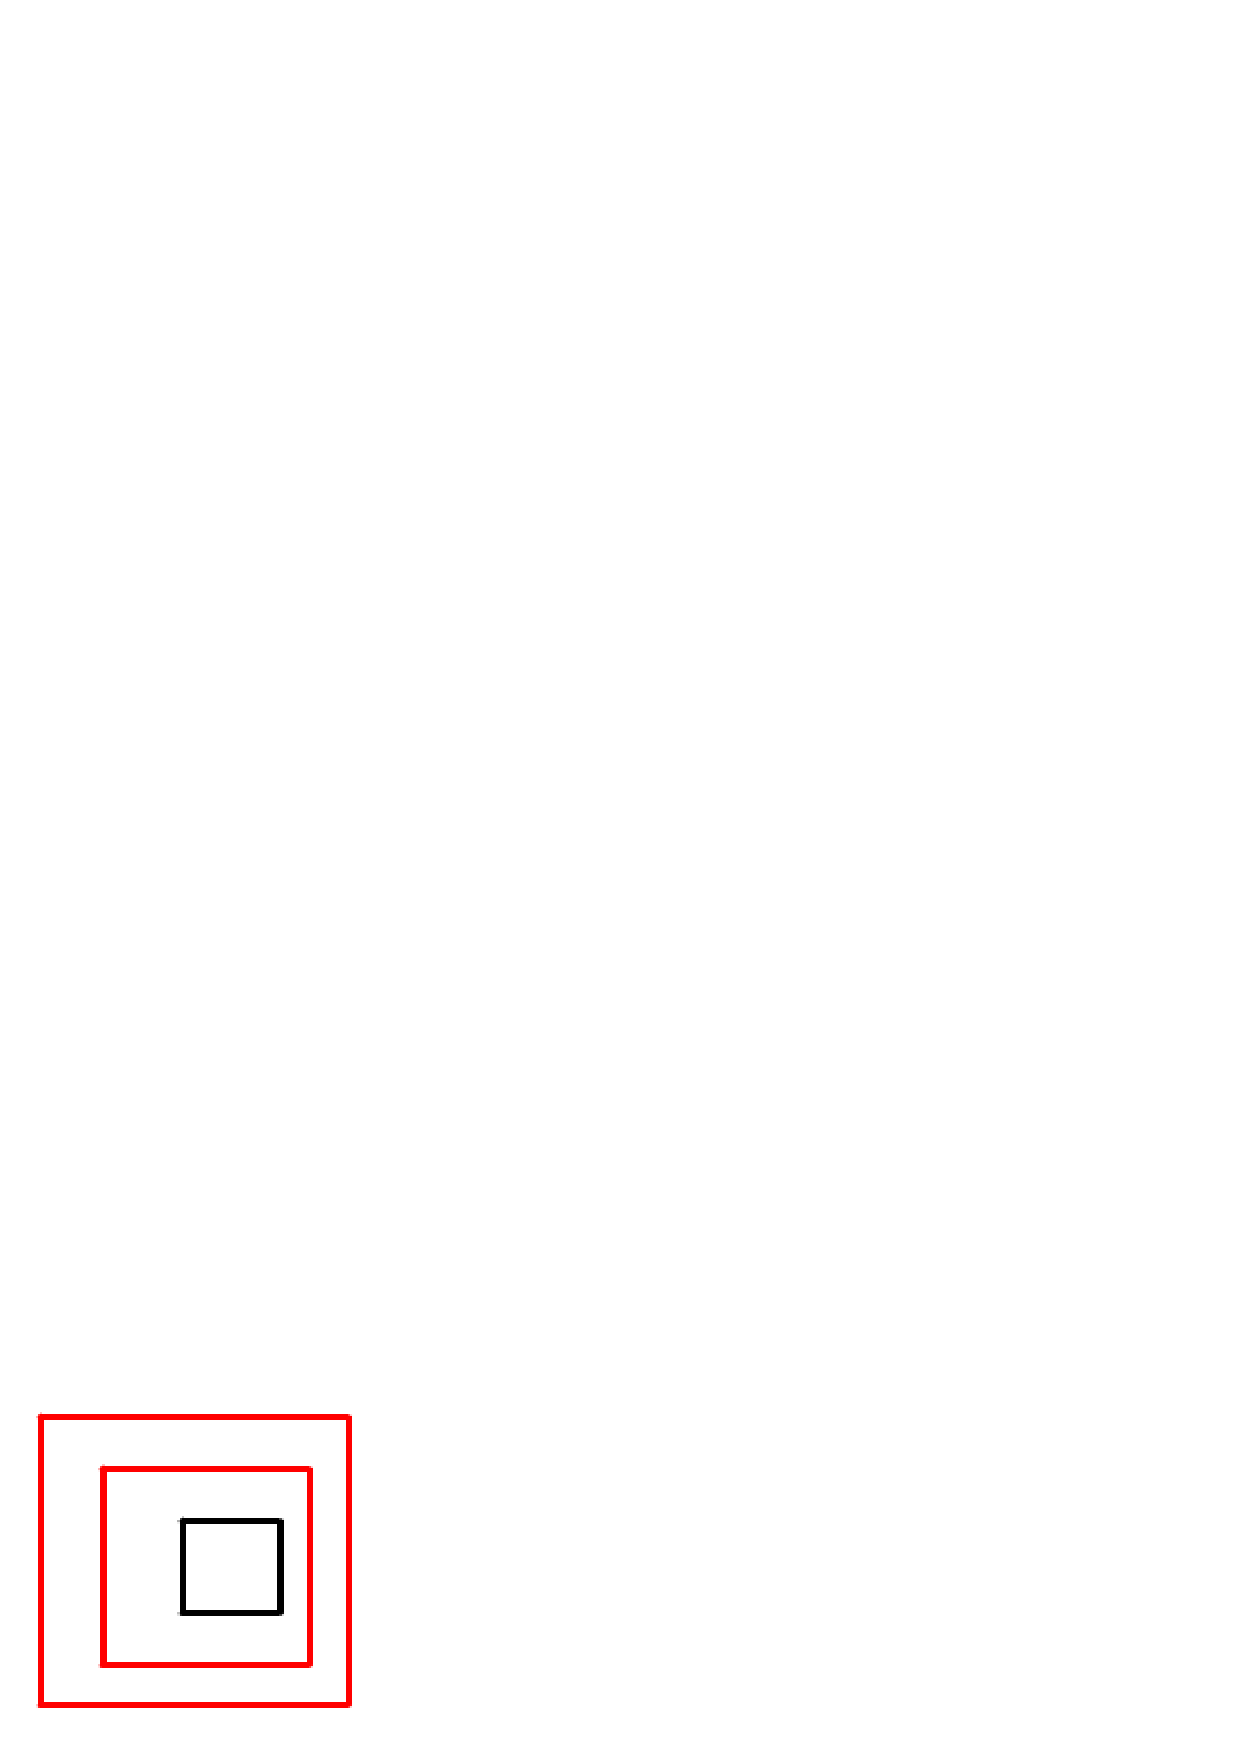
\includegraphics[scale=0.30]{img/QT8}
\caption{Superposition de boîtes}
\label{fig:superpos}
\end{figure}

\paragraph{Inconvénient de cette méthode}Le problème majeur de cette méthode se présente lorsque des boîtes sont côte à côte (cf : figure \ref{fig:frontiere}).
\begin{figure}[htbp]
\centering
\includegraphics[scale=0.40]{img/QT7}
\caption{Superposition de boîtes 1}
\label{fig:frontiere}
\end{figure}
Dans une telle situation chaque division va entraîner la création d'un espace dans la même configuration. L'algorithme ne s'arrêtera donc pas avant d'avoir atteint la taille minimale d'un espace. Nous nous retrouvons donc avec un grand nombre de boîtes au niveau de ces \og frontières\fg{} (cf : figure \ref{fig:frontiere2}).
\begin{figure}[htbp]
\centering
\includegraphics[scale=0.40]{img/QT9}
\caption{Superposition de boîtes 2}
\label{fig:frontiere2}
\end{figure}
Ainsi sachant que la précision maximale par défaut de \emph{RealPaver} est de $10^{-16}$, cela implique qu'il est nécessaire d'au moins égaler cette précision pour l'arbre de visualisation. Ainsi pour une sortie de \emph{RealPaver} contenant un total $l$ de longueurs de \og frontières \fg{}  cumulées et $p$ la précision du modèle, on a un nombre d'espaces à créer supérieur à $\frac{l}{p}$ avec $p$ très petit. Par exemple pour une sortie de \emph{RealPaver} comportant une \og frontière \fg{} de taille $1$, il faudra au moins $10^{16}$ espaces pour la contenir. 

\paragraph{Brève conclusion} Le QuadTree est une structure intéressante pour la visualisation mais si un nœud de l'arbre a un coût en mémoire non nul, alors l'espace mémoire de la structure va exploser. Elle semble donc, pour le moment, inappropriée.

\subsection{\'Etude d'une seconde solution : le R-tree}
\paragraph{}Bien que le QuadTree soit une structure intéressante pour permettre l'indexation et la recherche de points dans un espace, celui-ci l'est beaucoup moins pour la gestion de données à dimensions non nulles. Le R-tree est une structure proposé en 1984 par Antonin \textsc{Guttman} permettant l'indexation et la recherche d'éléments de dimension $d > 0$ dans $k$ dimensions\cite{Guttman}.

\paragraph{}Le R-tree est une variante équilibré de l'arbre B, sa structure est la suivante :
\begin{itemize}
 \item Un noeud de l'arbre correspond à une boîte non-solution du pavage. Chacun de ces nœuds est un MBR\footnote{\og \emph{Minimum bounding rectangle}\fg{} : les rectangles étant, dans le cas présent, $d$-dimensionnels.} de ces fils.
 \item Chaque boîte peut contenir entre $m$ et $M$ sous-boîtes entièrement incluses. Avec $m\leq \frac{M}{2}$.
 \item Une feuille de l'arbre est une boîte ne contenant que des boîtes solution du pavage.
\end{itemize}

La figure \ref{fig:rtree} donne une bonne idée de l'organisation des R-trees:
\begin{figure}[htbp]
\centering
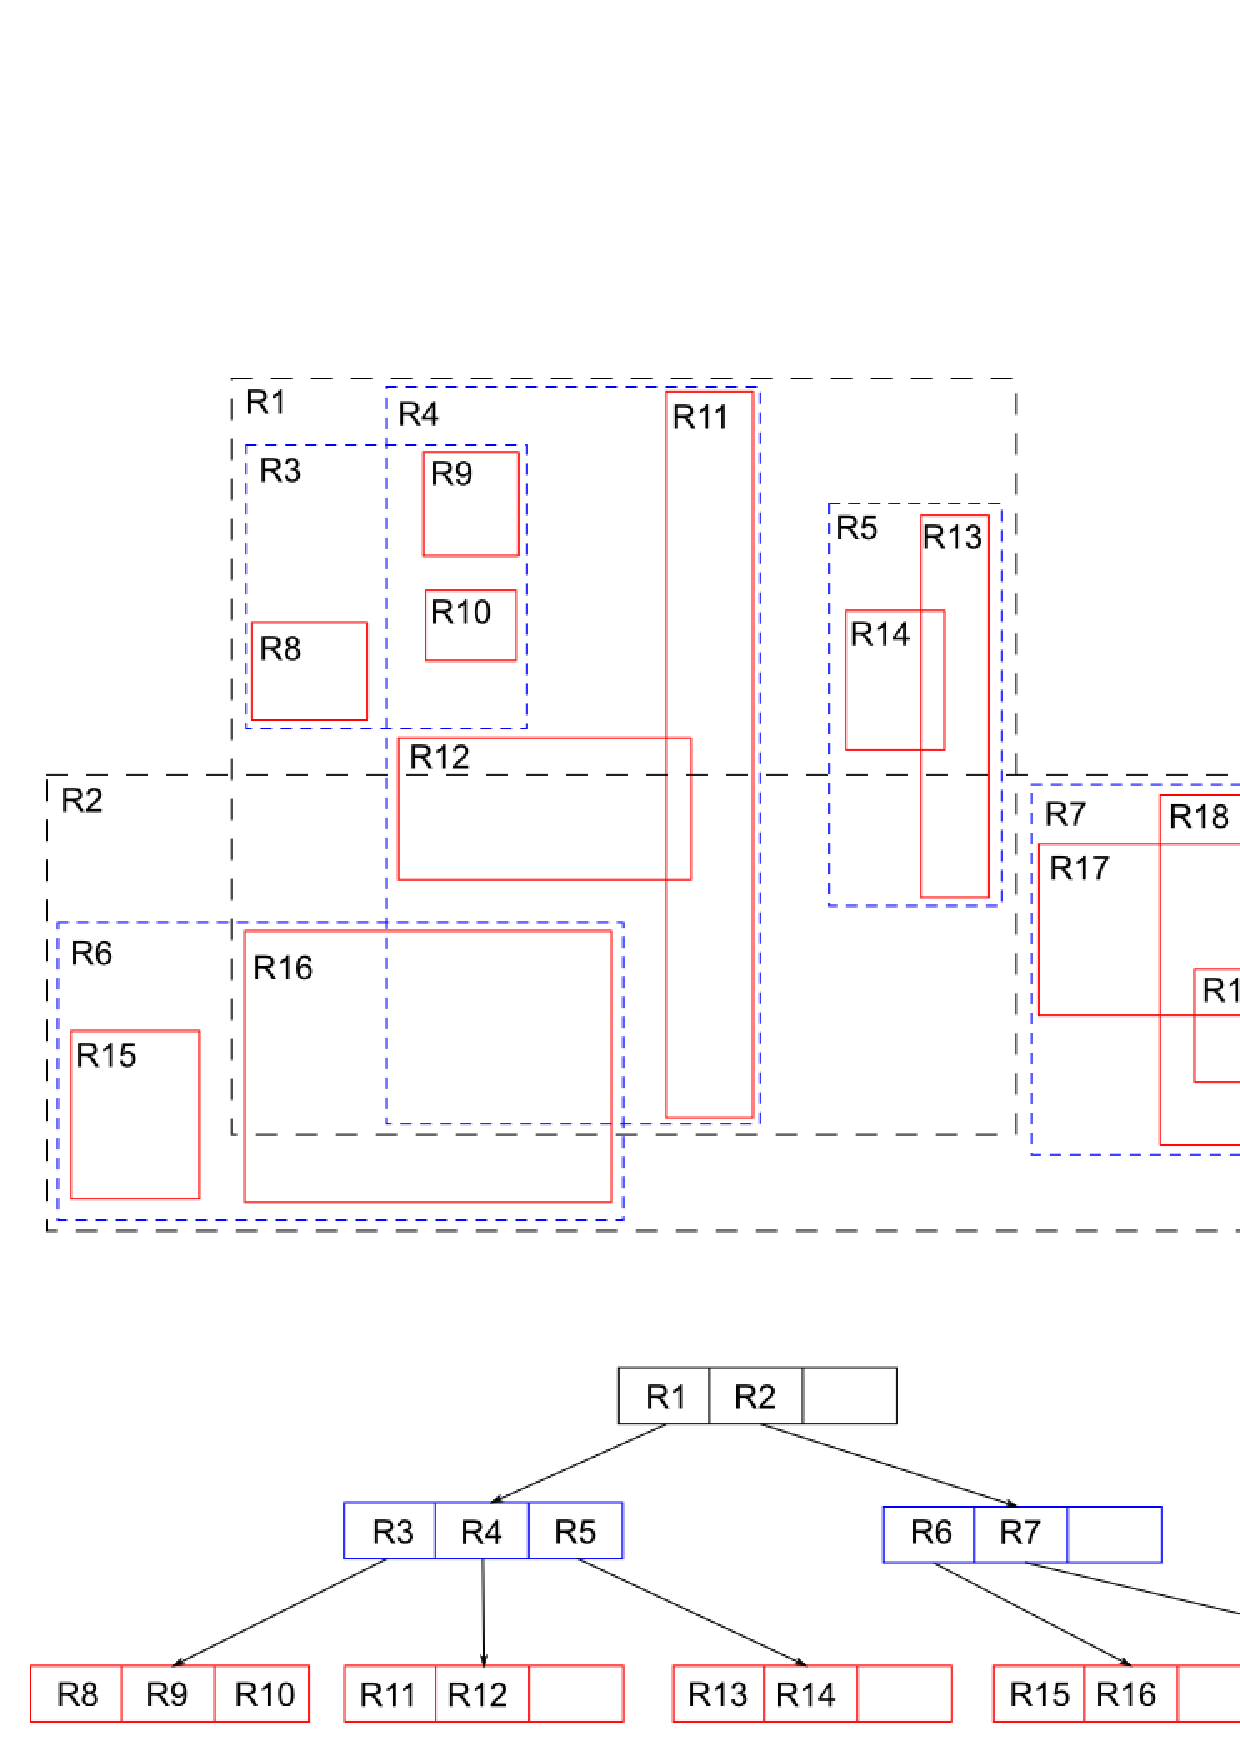
\includegraphics[scale=0.50]{img/rtree}
\caption{Représentation d'un R-tree\cite{wiki}}
\label{fig:rtree}
\end{figure}

Les algorithmes permettant la recherche et la création du R-tree sont quant à eux décrient dans l'article de \textsc{A. Guttman} dans la section \textbf{3. Searching and Updating}\cite{Guttman}. Nous rappelons brièvement les algorithmes de recherche (cf. Algorithme \ref{algo:recherche}) et d'ajout d'une boîte (cf. Algorithme \ref{algo:ajout}) \cite{poulos}.

\begin{algorithm}
%\caption{\textbf{Recherche}(nœud $N$, rectangle $R$)}
/* \textit{Recherche l'ensemble des feuilles contenues dans un rectangle requête $d$-dimensionnel à partir d'un nœud $N$, les feuilles solutions seront stockées dans $\Lambda$} */
\label{algo:recherche}
\begin{algorithmic}[1]
\IF {$N$ n'est pas une feuille}
  \FORALL{éléments $n$ de $N$ dont le MBR intersecte $R$}
    \STATE \textbf{Recherche}($n$, $R$)
  \ENDFOR
\ELSE[$N$ est une feuille] %\COMMENT{$N$ est une feuille}
  \FORALL{éléments $n$ de $N$ dont le MBR intersecte $R$}
    \STATE ajouter $n$ à $\Lambda$
  \ENDFOR
\ENDIF
\RETURN $\Lambda$
\end{algorithmic}
\end{algorithm}

\begin{algorithm}
\caption{\textbf{Ajout}(élément $E$, nœud $NR$)}
/* \textit{Ajoute un nouvel élément $E$ dans le R-tree de nœud racine $NR$} */
\label{algo:ajout}
\begin{algorithmic}[1]
\STATE On parcourt l'arbre depuis la racine $NR$ jusqu'à la feuille appropriée. À chaque niveau, on sélectionne le nœud dont le MBR nécessite le plus petit élargissement pour contenir le MBR de $E$
\STATE En cas d'égalité, on choisit le nœud ayant le MBR de plus petite \og superficie \fg{}
\IF{la feuille atteinte $L$ n'est pas pleine}
  \STATE On insère $E$ dans $L$
  \STATE On met à jour tous les MBR de $L$ jusqu'à $NR$ pour qu'ils puissent contenir le MBR de E 
\ELSE[la feuille $L$ est pleine]
  \STATE On définie $\xi$ l'ensemble constitué de tous les éléments de $L$ et du nouvel élément~$E$\\
On choisit deux éléments $e_1$ et $e_2$ tel que la distance entre $e_1$ et $e_2$ soit la plus grande de toutes les autres paires de $\xi$\\
On crée deux nœuds $l_1$ et $l_2$ contenant respectivement $e_1$ et $e_2$
  \STATE On parcourt tous les éléments restants de $\xi$ et l'on assigne chacun d'eux à $l_1$ ou $l_2$, en fonction du MBR de ces nœuds qui nécessitera le plus petit élargissement pour contenir le MBR de l'élément considéré
  \IF{égalité de l'élargissement}
    \STATE On assigne l'élément au nœud ayant le MBR de plus petite superficie
    \IF{égalité de superficie}
      \STATE On assigne l'élément au nœud ayant le moins d'élément
    \ENDIF
  \ENDIF
  \IF[On rappelle que m est le nombre minimal d'éléments que peut contenir un nœud]{Il reste $\lambda$ éléments dans $\xi$ et qu'un nœud contient $m - \lambda$ éléments}
    \STATE On assigne tous les éléments restants dans $\xi$ à ce nœud
  \ENDIF
  \STATE On met à jour le MBR des nœuds se trouvant sur le chemin de $L$ à $NR$ pour que ceux ci couvrent le MBR de $l_1$ et $l_2$
  \STATE On effectue les \og splits \fg{} éventuels des nœuds supérieurs
\ENDIF 
\end{algorithmic}
\end{algorithm}


\paragraph{Avantages et inconvénients du R-tree} Le R-tree est une structure de données spécialement conçue pour la recherche de données à dimensions $d$ pour dans des espaces $k$-dimensionnels. L'arbre a une profondeur maximale $h_{max}$ égale à :
\begin{equation}
 h_{max} = \left\lceil\log_{m} n\right\rceil - 1
\end{equation}
et le nombre de nœuds est au pire égale à :
\begin{equation}
 \sum_{i=1}^{h_{max}}{\left\lceil\frac{n}{m^i}\right\rceil} = \left\lceil\frac{n}{m}\right\rceil + \left\lceil\frac{n}{m^2}\right\rceil + \cdots + 1
\end{equation}

 Bien que ne pouvant garantir de bonnes performances en pire cas\footnote{\og \emph{More than one substree under a node may need to be searched, hence it is not possible to guarantee good worst-case performance.}\fg{}\cite{Guttman}, section \textbf{3.1 Searching}}, le R-tree offre en pratique de bons résultats ; on pourra d'ailleurs se reporter à l'analyse de performances effectuer par A. \textsc{Guttman}\footnote{section \textbf{4. Performance}\cite{Guttman}}. Cependant il existe aujourd'hui de nombreuses variantes du R-tree ( R*tree, Hilbert R-tree, etc\dots{} ), on pourra donc, pour une analyse plus générale des différentes implémentations, préférer \og\emph{R-trees : Theory and Applications} \fg{}\cite{poulos}.

\subsection{Conclusion}
Au vu de l'étude comparative entre les deux structures, le R-tree nous semble une structure plus adéquate pour répondre à une visualisation des pavages. En effet, bien que le QuadTree soit adapté pour stocker des éléments sans dimension, il devient moins performant et plus coûteux lorsque les éléments sont $d$-dimensionnels et notamment lorsque le pavage résultat possède un grand nombre de boîtes adjacentes comme c'est le cas pour la figure \ref{fig:DisqueDisque}. La structure R-tree quant à elle offre de meilleurs résultats sur les objets $d$-dimensionnels et semble donc plus adaptée pour notre logiciel de visualisation.


